%xelatex -shell-escape -output-directory=bin ergasia.tex
\documentclass{assignment}

\usepackage{enumerate} % Για την χρησιμοποίηση roman enumerate
\usepackage{paralist} % για το περιβάλλον inparaenum που είναι οι λίστες μέσα στο κείμενο.

\title{Δίκτυα Υπολογιστών \\ 1ο Εργαστήριο: Στατική Δρομολόγηση \\ Εργασία: assign2}
\date{Αθήνα, 2015}

\author{Αναγνωστόπουλος Βασίλης - Θάνος (ΜΠΠΛ 13002) \and Βελισσαρίου Κυριάκος (ΜΠΠΛ 13005)}

\begin{document}

\maketitle
% Να σκεφτώ τί αλλαγές θέλω να κάνω με τις αριθμήσεις και άμα θέλω να κάνω.
% Να σκεφτώ να τις ενσωματώσω και στο assignment.cls

\setcounter{page}{1} 
\pagenumbering{roman}

\pagestyle{plain}
\tableofcontents
\listoftables
\listoffigures
%\renewcommand\listoflistingscaption{Κατάλογος πηγαίου κώδικα}
%\listoflistings
\newpage

%\pagestyle{headings}
%\pagestyle{fancy}
\setcounter{page}{1} 
\pagenumbering{arabic}


Δίνεται η παρακάτω τοπολογία:

\begin{center}
\resizebox*{\textwidth}{!}{
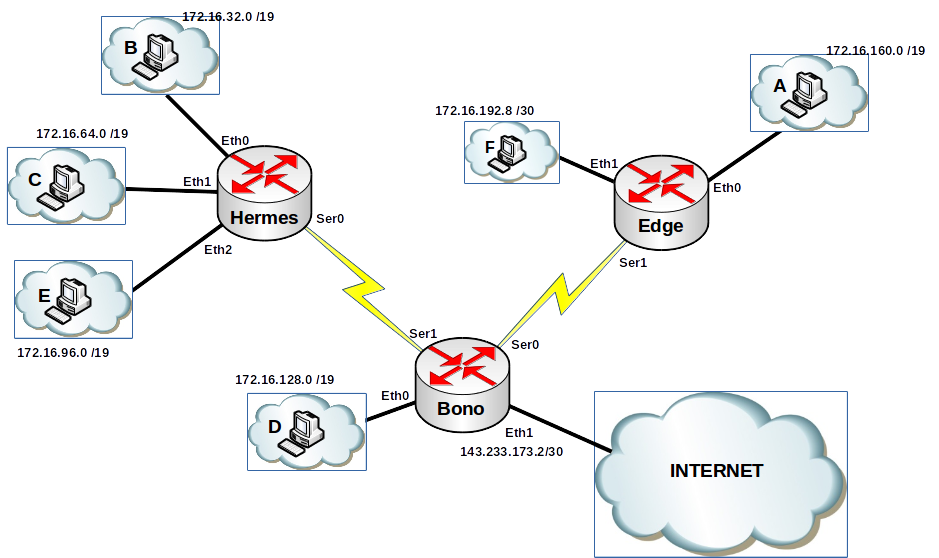
\includegraphics{images/lan.png}}
\end{center}
 
Παραδοτέα:

\begin{enumerate}
  \item Η έκθεση σας:
  \begin{enumerate}
     \item Screenshot της τοπολογίας.
     \item Screenshot που θα εμφανίζει τις επιτυχημένες προσπάθειες πρόσβασης 2 σταθμών στην υπηρεσία HTTP.
     \item Screenshot που θα αποδεικνύει το ζητούμενο 3, όπως διατυπώνεται παραπάνω.
     \item Screenshot με το αποτέλεσμα εκτέλεσης της εντολής \#show ip ospf
     \item Screenshot με το αποτέλεσμα εκτέλεσης της εντολής \#show ip ospf database
  \end{enumerate}
  \item Τα αρχεία (.pkt) με την τοπολογία σας.
\end{enumerate}

Ζητούμενα:


\section{Άσκηση 1η}
\subsection{Εκφώνηση}

Υλοποιήστε την τοπολογία με το λογισμικό που σας δόθηκε. Σε περιπτώσεις όπου δεν δίνονται IP διευθύνσεις, θα πρέπει να υπολογισθούν από εσάς και να αποδοθούν στα αντίστοιχα interface των δρομολογητών. Σημειώστε ότι οι δοθείσες IP διευθύνσεις ανταποκρίνονται στις IP των δικτύων της τοπολογίας – εξαιρείται η διεύθυνση IP του eth1 του δρομολογητή Bono. 

\subsection{Λύση}


Βρίσκουμε τη μάσκα υποδικτύωσης και το εύρος των διευθύνσεων για κάθε υποδίκτυο (βλ. πίνακα \ref{table:VLSM_subnetting}):

\begin{description}
\item[SubnetA έως SubnetE:] H μάσκα υποδικτύωσης είναι $/19$ $(32-13)$ ή 255.255.224.0 Στο υποδίκτυο εκτός από την διεύθυνση υποδικτύου και την \en{broadcast} διεύθυνση θα υπάρχουν $2^{19} - 2 = 8190$ διευθύνσεις για τους \en{hosts}. Συνολικά δηλαδή σε κάθε υποδίκτυο θα υπάρχουν $2^{19} = 8192$ διευθύνσεις.

\item[SubnetF:] H μάσκα υποδικτύωσης είναι $/30$ $(32-2)$ ή 255.255.255.252. Στο υποδίκτυο εκτός από την διεύθυνση υποδικτύου και την \en{broadcast} διεύθυνση θα υπάρχουν 2 διευθύνσεις για τους \en{hosts}. Συνολικά δηλαδή σε κάθε υποδίκτυο θα υπάρχουν $2^2 = 4$ διευθύνσεις.

\item[SubnetSer1:] Θα πρέπει να αποδοθούν IP και στα interface των σειριακών συνδέσεων. Άρα θα χρησιμοποιήσουμε το μικρότερο δυνατό υποδίκτυο. Άρα πρέπει $2^y -2 \geq 2$. Άρα $y=2$ οπότε η μάσκα υποδικτύωσης θα είναι $/30$ $(32-2)$ ή 255.255.255.252. Στο υποδίκτυο εκτός από την διεύθυνση υποδικτύου και την \en{broadcast} διεύθυνση θα υπάρχουν 2 διευθύνσεις για τους \en{hosts}. Συνολικά δηλαδή σε κάθε υποδίκτυο θα υπάρχουν 4 διευθύνσεις.

\item[SubnetSer2:] Ομοίως πρέπει $2^y -2 \geq 2$. Άρα $y=2$ οπότε η μάσκα υποδικτύωσης θα είναι $/30$ $(32-2)$ ή 255.255.255.252. Στο υποδίκτυο εκτός από την διεύθυνση υποδικτύου και την \en{broadcast} διεύθυνση θα υπάρχουν 2 διευθύνσεις για τους \en{hosts}. Συνολικά δηλαδή σε κάθε υποδίκτυο θα υπάρχουν 4 διευθύνσεις.

\item[Internet:] Και το interface που συνδέεται στο ίντερνετ θα πρέπει να ανήκει σε κάποιο υποδίκτυο. Επειδή δεν δίνεται κάποια άλλη πληροφορία θα θεωρεί ότι είναι το μικρότερο δυνατό. Άρα πρέπει $2^y -2 \geq 2$. Άρα $y=2$ οπότε η μάσκα υποδικτύωσης θα είναι $/30$ $(32-2)$ ή 255.255.255.252. Στο υποδίκτυο εκτός από την διεύθυνση υποδικτύου και την \en{broadcast} διεύθυνση θα υπάρχουν 2 διευθύνσεις για τους \en{hosts}. Συνολικά δηλαδή σε κάθε υποδίκτυο θα υπάρχουν 4 διευθύνσεις.


\end{description}


\begin{table}
\begin{center}
  \begin{tabular}{|m{2.3cm}|m{2.9cm}|m{3.5cm}|m{3.4cm}|m{3.3cm}|}
    \hline
    Subnet & Subnet Address & Subnet Mask & Host Addresses & BroadCast Address \\ \hline
  SubnetA & 172.16.160.0 & 255.255.224.0 & 172.16.160.1 - 172.16.191.254 & 172.16.191.255 \\ \hline
  SubnetB & 172.16.32.0 & 255.255.224.0 & 172.16.32.1 - 172.16.63.254 & 172.16.63.255 \\ \hline
  SubnetC & 172.16.64.0 & 255.255.224.0 & 172.16.64.1 - 172.16.95.254 & 172.16.95.255 \\ \hline
  SubnetD & 172.16.128.0 & 255.255.224.0 & 172.16.128.1 - 172.16.159.254 & 172.16.159.255 \\ \hline
  SubnetE & 172.16.96.0 & 255.255.224.0 & 172.16.96.1 - 172.16.127.254 & 172.16.127.255 \\ \hline
  SubnetF & 172.16.192.8 & 255.255.255.252 & 172.16.192.9 - 172.16.192.10 & 172.16.192.11 \\ \hline
  SubnetSer1 & 172.16.192.0 & 255.255.255.252 & 172.16.192.1 - 172.16.192.2 & 172.16.192.3 \\ \hline
  SubnetSer2 & 172.16.192.4 & 255.255.255.252 & 172.16.192.5 - 172.16.192.6 & 172.16.192.7 \\ \hline
  SubnetInt & 143.233.173.0 & 255.255.255.252 & 143.233.173.1 - 143.233.173.2 & 143.233.173.3 \\ \hline


  
  \end{tabular}
\caption{Ο πίνακας των υποδικτύων του δικτύου.}
\label{table:VLSM_subnetting}
\end{center}
\end{table}

Για την απόδοση των ΙΡ διευθύνσεων ακολουθήθηκαν τα παρακάτω:
\begin{itemize}
\item Για τις διεπαφές των δρομολογητών η απόδοση των ΙΡ διευθύνσεων να αρχίζει από την τελευταία έγκυρη Host IP διεύθυνση του εκάστοτε υποδικτύου, με φθίνουσα σείρα.
\item Για τις διεπαφές των υπόλοιπων δικτυακών συσκευών η απόδοση των ΙΡ
διευθύνσεων να αρχίζει από την πρώτη έγκυρη Host IP διεύθυνση του εκάστοτε
υποδικτύου, με αύξουσα σειρά.
\end{itemize}

Από τους παραπάνω κανόνες προέκυψε ο πίνακας \ref{table:VLSM_ip}.

\begin{table}
\begin{minipage}{\textwidth} 
\begin{center}
  \begin{tabular}{|c|c|c|c|c|}
    \hline
    Device & Interface & IP Address & Subnet Mask & Default Gateway \\ \hline
    \multirow{4}{*}{Hermes} &  Fa9/0 & 172.16.63.254 & 255.255.224.0 & - \\ \cline{2-5}
                            &  Fa8/0 & 172.16.95.254 & 255.255.224.0 & - \\ \cline{2-5}
                            &  Fa7/0 & 172.16.127.254 & 255.255.224.0 & - \\ \cline{2-5}
                            &  Ser0/0 & 172.16.192.2 & 255.255.255.252 & - \\ \hline

    \multirow{4}{*}{Bono}   &  Fa9/0 & 172.16.159.254 & 255.255.224.0 & - \\ \cline{2-5}
                            &  Fa8/0 & 143.233.173.2 & 255.255.255.252 & - \\ \cline{2-5}
                            &  Ser0/0 & 172.16.192.1 & 255.255.255.252 & - \\ \cline{2-5}
                            &  Ser1/0 & 172.16.192.6 & 255.255.255.252 & - \\ \hline

    \multirow{4}{*}{Edge}   &  Fa8/0 & 172.16.191.254 & 255.255.224.0 & - \\ \cline{2-5}
                            &  Fa9/0 & 172.16.192.10 & 255.255.255.252 & - \\ \cline{2-5}
                            &  Ser0/0 & 172.16.192.5 & 255.255.255.252 & - \\  \hline

    PCA & Eth & 172.16.160.1 & 255.255.224.0 & 172.16.191.254 \\ \hline
    PCB & Eth & 172.16.32.1 & 255.255.224.0 & 172.16.63.254 \\ \hline
    PCC & Eth & 172.16.64.1 & 255.255.224.0 & 172.16.95.254 \\ \hline
    PCD & Eth & 172.16.128.1 & 255.255.224.0 & 172.16.159.254 \\ \hline
    PCE & Eth & 172.16.96.1 & 255.255.224.0 & 172.16.127.254 \\ \hline
    PCF & Eth & 172.16.192.9 & 255.255.255.252 & 172.16.192.10 \\ \hline
  \end{tabular}
\caption{Ο πίνακας των ip διευθύνσεων του δικτύου.}
\label{table:VLSM_ip}
\end{center}
\end{minipage}
\end{table}

Η υλοποίηση στο \en{Cisco Packet Tracer} φαίνεται στο σχήμα \ref{fig:cisco}.

%\begin{figure}
%\begin{center}
%\resizebox*{\textwidth}{!}{
%\includegraphics{images/cisco.png}}
%\caption{Η υλοποίηση του δικτύου στο \en{Cisco Packet Tracer}}
%\label{fig:cisco}
%\end{center}
%\end{figure}


\section{Άσκηση 2η}
\subsection{Εκφώνηση}

Όλοι οι σταθμοί της τοπολογίας πρέπει να έχουν πρόσβαση στην υπηρεσία HTTP που εξυπηρετείται από κάποιον διακομιστή στο Διαδίκτυο. Δεν έχουν πρόσβαση σε κάποια άλλη υπηρεσία του διαδικτύου.

\subsection{Λύση}


\section{Άσκηση 3η}
\subsection{Εκφώνηση}

Τα δίκτυα που βρίσκονται στον δρομολογητή Hermes είναι προσβάσιμα σε όλους τους άλλους μόνο σε περίπτωση χρήσης των εργαλείων ping και traceroute.

\subsection{Λύση}

\section{Άσκηση 4η}
\subsection{Εκφώνηση}

Οι δρομολογητές αξιοποιούν τον αλγόριθμο OSPF για τη διαδικασία της δρομολόγησης. 
Προς το Διαδίκτυο χρησιμοποιείται στατική δρομολόγηση.

\subsection{Λύση}

\captionof{listing}{Οι εντολές για το OSPF στον Hermes}
\begin{minted}[breaklines=true, frame=lines, framesep=2mm, baselinestretch=1.2, fontsize=\footnotesize, linenos]{bash}
Hermes(config)# router ospf 500
Hermes(config-router)# network 172.16.32.0 0.0.31.255 area 0
Hermes(config-router)# network 172.16.64.0 0.0.31.255 area 0
Hermes(config-router)# network 172.16.96.0 0.0.31.255 area 0
Hermes(config-router)# network 172.16.192.0 0.0.0.3 area 0
Hermes(config-router)# ^Z
Hermes(config)# ip route 143.233.173.0 255.255.255.252 172.16.192.1
\end{minted}

\captionof{listing}{Οι εντολές για το OSPF στον Edge}
\begin{minted}[breaklines=true, frame=lines, framesep=2mm, baselinestretch=1.2, fontsize=\footnotesize, linenos]{bash}
Edge(config)# router ospf 500
Edge(config-router)# network 172.16.192.8 0.0.0.3 area 0
Edge(config-router)# network 172.16.160.0 0.0.31.255 area 0
Edge(config-router)# network 172.16.192.4 0.0.0.3 area 0
Edge(config-router)# ^Z
Edge(config)# ip route 143.233.173.0 255.255.255.252 172.16.192.6
\end{minted}

\captionof{listing}{Οι εντολές για το OSPF στον Bono}
\begin{minted}[breaklines=true, frame=lines, framesep=2mm, baselinestretch=1.2, fontsize=\footnotesize, linenos]{bash}
Bono(config)# router ospf 500
Bono(config-router)# network 172.16.128.0 0.0.31.255 area 0
Bono(config-router)# network 172.16.192.0 0.0.0.3 area 0
Bono(config-router)# network 172.16.192.4 0.0.0.3 area 0
\end{minted}

\phantomsection \label{Βιβλιογραφία}
\addcontentsline{toc}{section}{Βιβλιογραφία}
%\mtcaddchapter[Βιβλιογραφία] % Λόγω του minitoc
\bibliographystyle{plain}
\bibliography{references}

\newpage

\end{document}

